Na wykresie \ref{fig:JumpingValues} przedstawiono przykładowy przebieg wartości dla pierwszych 5 zmian
wraz z zaznaczonymi miejscami,
gdzie nastąpiła.
\begin{figure}[htbp]
  \centering
  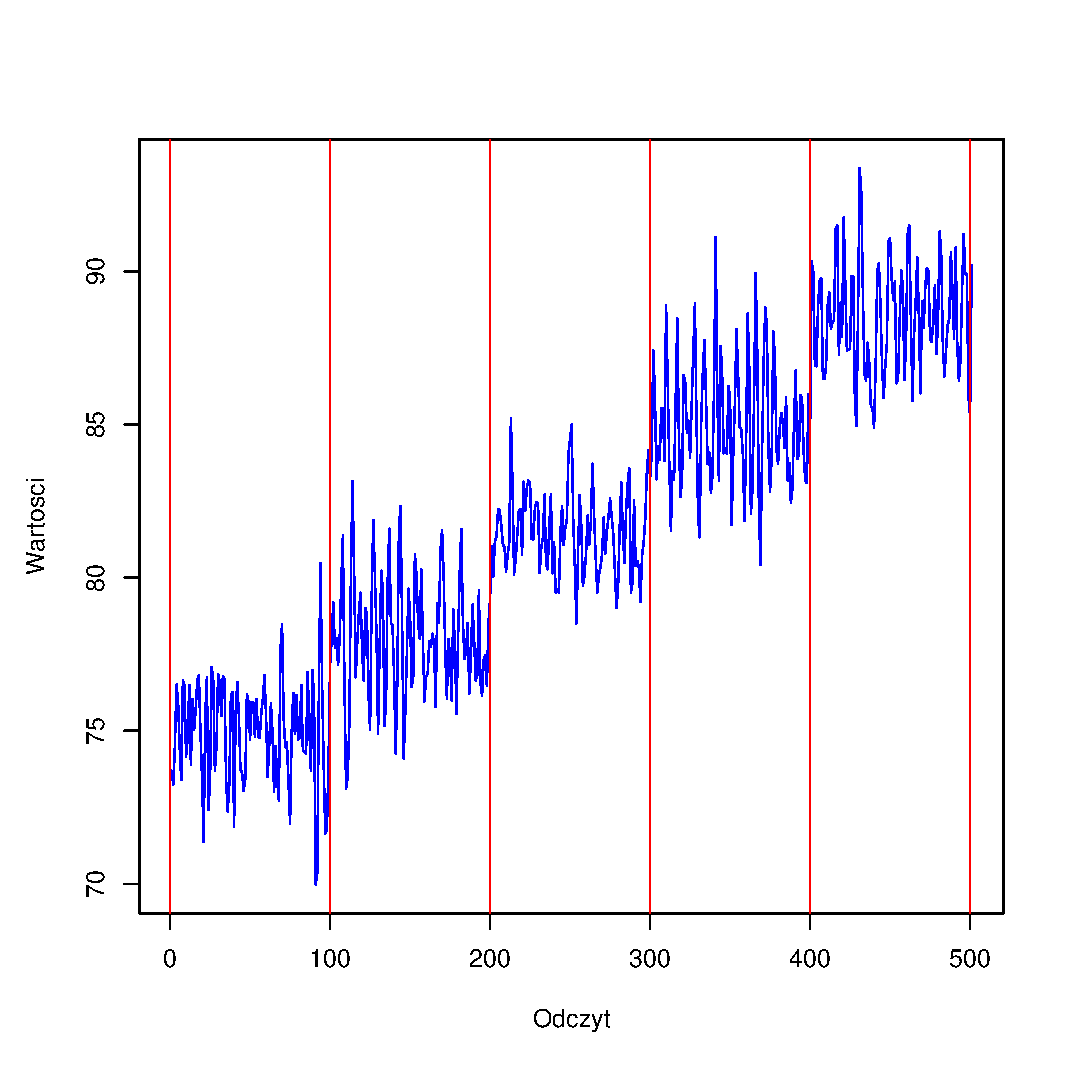
\includegraphics[width=0.5\textwidth]{img/ch-5-jumping}
  \caption{Przykładowe wartości}
  \label{fig:JumpingValues}
\end{figure}
Badanie przeprowadzono poprzez wygenerowanie 20 zestawów danych.
Źródło (\textit{seed}) dla każdego z zestawów były inne.

Na wykresach \ref{fig:JumpingValuesResTpr} i \ref{fig:JumpingValuesResNpr} przedstawion otrzymane wyniki.
Na osi OX zaznaczono kolejne przeprowadzone próby.
Na osi OY przedstawiono odpowiednio współczynnik suksesów (TPR) i fałszywe alarmy (NPR).
Jeśli chodzi o skuteczność (TPR) widać wyraźną przewagę algorytmów z rodziny ADWIN.
Praktycznie w każdej z prób częsciej wykrywały zajście zmiany.
Różnice pomiędzy $ADWIN_d$,
a $ADWIN_{\mu}$ są niezauważalne i z powodzeniem można korzystać z obu.
Niestety jeśli chodzi generowanie fałszywych alarmów wszystkie badane algorytmy
mają zbliżony do siebie poziom.

Zbiorcze wyniki testów przedstawono w tabeli \ref{tab:JumpingResult}.
\begin{table}[h]
  \label{tab:JumpingResult}
  \centering
  \begin{tabular}{l r r r r}
    & \multicolumn{2}{l}{TPR} & \multicolumn{2}{l}{NPR} \\
    \hline
    & \multicolumn{1}{l}{Średnia} & \multicolumn{1}{l}{Wariancja}& \multicolumn{1}{l}{Średnia} & \multicolumn{1}{l}{Wariancja} \\
    \hline
    BAY & 0,439 & $0,887 \times 10^{-3}$ & 0,689 & $1,213 \times 10^{-3}$  \\
    $ADW_{\mu}$ & 0,526 & $1,246 \times 10^{-3}$ & 0,727 & $1,539 \times 10^{-3}$ \\
    $ADW_{d}$ & 0,516 & $2,508 \times 10^{-3}$ & 0,712 & $2,627 \times 10^{-3}$ \\
  \end{tabular}
  \caption{Zbiorcze wyniki testów}
\end{table}

\begin{figure}[htbp]
  \centering
  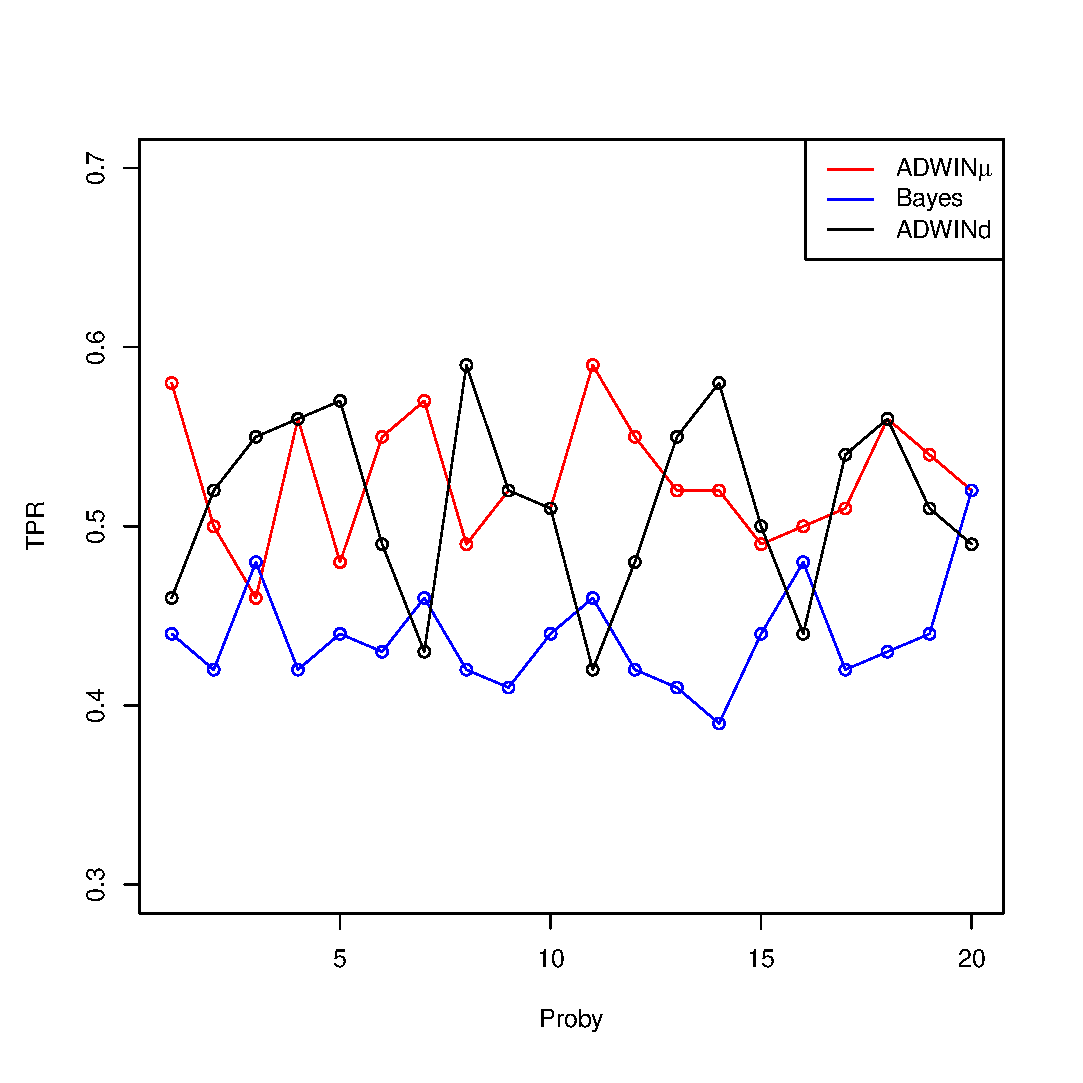
\includegraphics[width=0.6\textwidth]{img/ch-5-jump-res-tpr}
  \caption{Wyniki dla poszczególnych prób -- współczynnik suksesów}
  \label{fig:JumpingValuesResTpr}
\end{figure}
\begin{figure}[htbp]
  \centering
  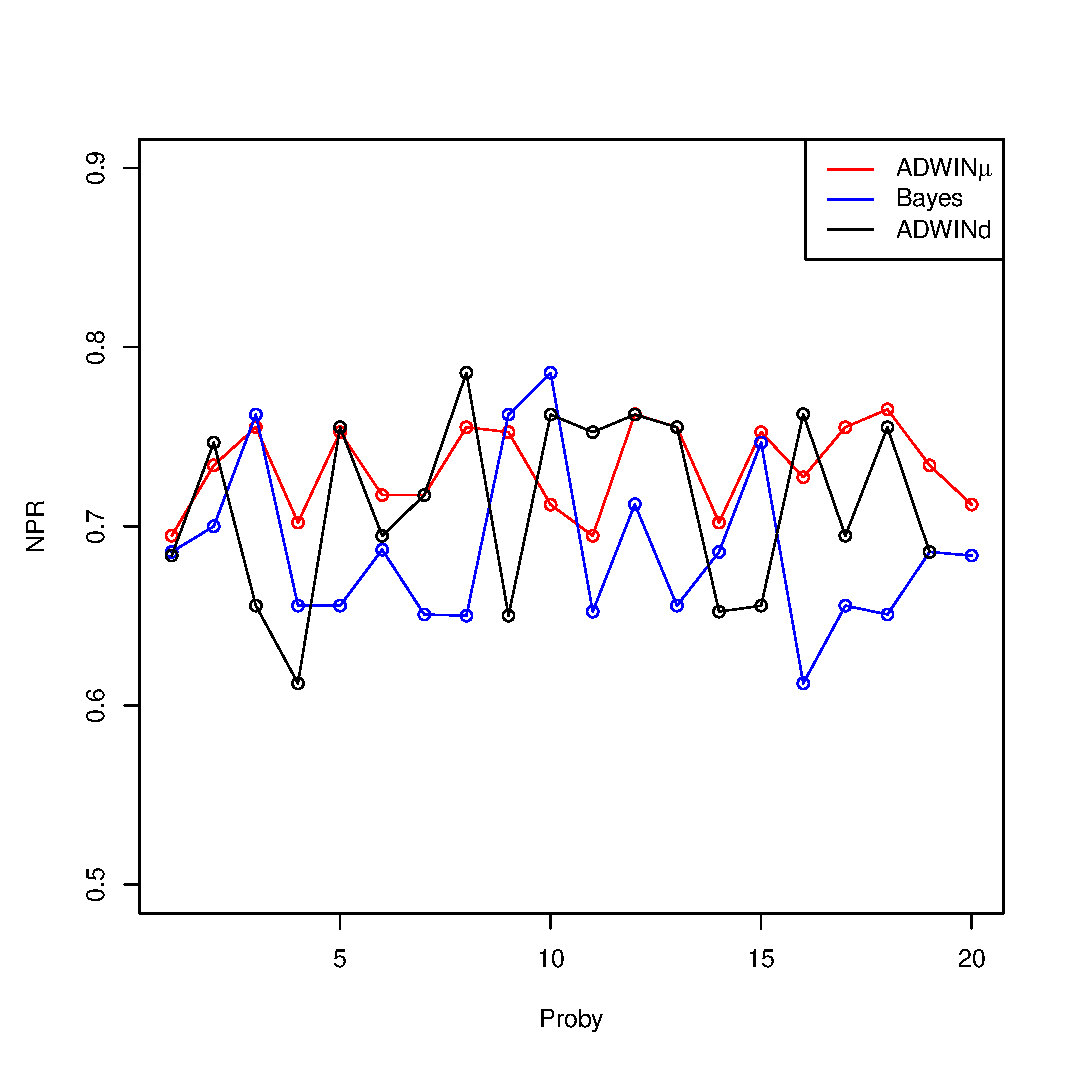
\includegraphics[width=0.6\textwidth]{img/ch-5-jump-res-npr}
  \caption{Wyniki dla poszczególnych prób -- współczynnik fałszywych alarmów}
  \label{fig:JumpingValuesResNpr}
\end{figure}
